\documentclass[a4paper,oneside,12pt]{extreport}

\usepackage{mmap}
\usepackage[T2A]{fontenc}
\usepackage[utf8]{inputenc}
\usepackage[english,russian]{babel}

\renewcommand{\ttdefault}{PTMono-TLF}

% Текст отчёта следует печатать, соблюдая следующие размеры полей:
% левое — 30 мм, правое — 15 мм, верхнее и нижнее — 20 мм.
\usepackage[left=20mm, right=15mm, top=15mm, bottom=15mm]{geometry}

% \setlength{\parindent}{1.25cm} % Абзацный отступ

\usepackage{setspace}
% \onehalfspacing % Полуторный интервал

\frenchspacing % Равномерные пробелы
\usepackage{indentfirst} % Красная строка

\usepackage{microtype}
\sloppy

\usepackage{titlesec}
\titlespacing*{\chapter}{0pt}{-30pt}{8pt}
\titlespacing*{\section}{\parindent}{*4}{*4}
\titlespacing*{\subsection}{\parindent}{*4}{*4}
\titleformat{\chapter}{\LARGE\bfseries}{\thechapter}{20pt}{\LARGE\bfseries}
\titleformat{\section}{\Large\bfseries}{\thesection}{40pt}{\Large\bfseries}

\usepackage{graphicx}
\usepackage{caption}
\usepackage{float}

\usepackage[unicode,pdftex]{hyperref}
\hypersetup{hidelinks}

%% begin title
\usepackage{wrapfig}

\makeatletter
	\def\vhrulefill#1{\leavevmode\leaders\hrule\@height#1\hfill \kern\z@}
\makeatother
%% end title

%% begin code
\usepackage{listings}
\usepackage{listingsutf8}
\usepackage{xcolor}

\lstset{language=Matlab,%
    %basicstyle=\color{red},
    breaklines=true,%
    morekeywords={matlab2tikz},
    keywordstyle=\color{blue},%
    morekeywords=[2]{1}, keywordstyle=[2]{\color{black}},
    identifierstyle=\color{black},%
    stringstyle=\color{mylilas},
    commentstyle=\color{mygreen},%
    showstringspaces=false,%without this there will be a symbol in the places where there is a space
    numbers=left,%
    numberstyle={\tiny \color{black}},% size of the numbers
    numbersep=9pt, % this defines how far the numbers are from the text
    emph=[1]{for,end,break},emphstyle=[1]\color{red}, %some words to emphasise
    %emph=[2]{word1,word2}, emphstyle=[2]{style},    
    literate={Ö}{{\"O}}1
    {Ä}{{\"A}}1
    {Ü}{{\"U}}1
    {ß}{{\ss}}1
    {ü}{{\"u}}1
    {ä}{{\"a}}1
    {ö}{{\"o}}1
    {~}{{\textasciitilde}}1
    {а}{{\selectfont\char224}}1
    {б}{{\selectfont\char225}}1
    {в}{{\selectfont\char226}}1
    {г}{{\selectfont\char227}}1
    {д}{{\selectfont\char228}}1
    {е}{{\selectfont\char229}}1
    {ё}{{\"e}}1
    {ж}{{\selectfont\char230}}1
    {з}{{\selectfont\char231}}1
    {и}{{\selectfont\char232}}1
    {й}{{\selectfont\char233}}1
    {к}{{\selectfont\char234}}1
    {л}{{\selectfont\char235}}1
    {м}{{\selectfont\char236}}1
    {н}{{\selectfont\char237}}1
    {о}{{\selectfont\char238}}1
    {п}{{\selectfont\char239}}1
    {р}{{\selectfont\char240}}1
    {с}{{\selectfont\char241}}1
    {т}{{\selectfont\char242}}1
    {у}{{\selectfont\char243}}1
    {ф}{{\selectfont\char244}}1
    {х}{{\selectfont\char245}}1
    {ц}{{\selectfont\char246}}1
    {ч}{{\selectfont\char247}}1
    {ш}{{\selectfont\char248}}1
    {щ}{{\selectfont\char249}}1
    {ъ}{{\selectfont\char250}}1
    {ы}{{\selectfont\char251}}1
    {ь}{{\selectfont\char252}}1
    {э}{{\selectfont\char253}}1
    {ю}{{\selectfont\char254}}1
    {я}{{\selectfont\char255}}1
    {А}{{\selectfont\char192}}1
    {Б}{{\selectfont\char193}}1
    {В}{{\selectfont\char194}}1
    {Г}{{\selectfont\char195}}1
    {Д}{{\selectfont\char196}}1
    {Е}{{\selectfont\char197}}1
    {Ё}{{\"E}}1
    {Ж}{{\selectfont\char198}}1
    {З}{{\selectfont\char199}}1
    {И}{{\selectfont\char200}}1
    {Й}{{\selectfont\char201}}1
    {К}{{\selectfont\char202}}1
    {Л}{{\selectfont\char203}}1
    {М}{{\selectfont\char204}}1
    {Н}{{\selectfont\char205}}1
    {О}{{\selectfont\char206}}1
    {П}{{\selectfont\char207}}1
    {Р}{{\selectfont\char208}}1
    {С}{{\selectfont\char209}}1
    {Т}{{\selectfont\char210}}1
    {У}{{\selectfont\char211}}1
    {Ф}{{\selectfont\char212}}1
    {Х}{{\selectfont\char213}}1
    {Ц}{{\selectfont\char214}}1
    {Ч}{{\selectfont\char215}}1
    {Ш}{{\selectfont\char216}}1
    {Щ}{{\selectfont\char217}}1
    {Ъ}{{\selectfont\char218}}1
    {Ы}{{\selectfont\char219}}1
    {Ь}{{\selectfont\char220}}1
    {Э}{{\selectfont\char221}}1
    {Ю}{{\selectfont\char222}}1
    {Я}{{\selectfont\char223}}1
    {і}{{\selectfont\char105}}1
    {ї}{{\selectfont\char168}}1
    {є}{{\selectfont\char185}}1
    {ґ}{{\selectfont\char160}}1
    {І}{{\selectfont\char73}}1
    {Ї}{{\selectfont\char136}}1
    {Є}{{\selectfont\char153}}1
    {Ґ}{{\selectfont\char128}}1
}

%% end code

%% begin theorem
\usepackage{amsthm}

\makeatletter
\newtheoremstyle{indented}
	{}% measure of space to leave above the theorem
	{}% measure of space to leave below the theorem
	{}% name of font to use in the body of the theorem
	{\parindent}% measure of space to indent
	{\bfseries}% name of head font
	{.}% punctuation between head and body
	{ }% space after theorem head; " " = normal interword space
	{}% header specification (empty for default)
\makeatother

\theoremstyle{indented}

\newtheorem{definition}{Определение}[section]
\newtheorem{remark}{Замечание}[section]
%% end theorem


\usepackage{amsmath, amsfonts, amssymb}

\renewcommand\thesection{\arabic{section}}
\renewcommand\thesubsection{\thesection.\arabic{subsection}}

\begin{document}
\setcounter{page}{2}
\paragraph{Цель работы:} построение гистограммы и эмпирической функции распределения.

\paragraph{Содержание работы}

\begin{enumerate}
	\item Для выборки объёма $n$ из генеральной совокупности $X$ реализовать в виде программы на ЭВМ:
	\begin{itemize}
		\item вычисление максимального значения $M_{\max}$ и минимального значения $M_{\min}$,
		\item размаха $R$ выборки,
		\item вычисление оценок $\hat\mu$ и $S^2$ математического ожидания $MX$ и дисперсии $DX$,
		\item группировку значений выборки в $m = [\log_2 n] + 2$ интервала,
		\item построение на одной координатной плоскости гистограммы и графика функции плотности распределения вероятностей нормальной случайной величины с математическим ожиданием $\hat{\mu}$ и дисперсией $S^2$,
		\item построение на другой координатной плоскости графика эмпирической функции распределения и функции распределения нормальной случайной величины с математическим ожиданием $\hat{\mu}$ и дисперсией $S^2$.
	\end{itemize}
	\item Провести вычисления и построить графики для выборки из индивидуального варианта.
\end{enumerate}

\pagebreak
\section{Вариант 21, выборка}
$\vec{x} = ( 

~~~~~~~-14.34, -16.97, -14.09, -14.74, -16.69, -13.85, -15.55, -14.62, -13.30, -15.52,

~~~~~~~-14.75, -16.51, -17.15, -16.87, -15.06, -13.60, -14.48, -14.71, -14.17, -13.88,

~~~~~~~-14.55, -15.37, -14.81, -16.05, -17.06, -15.86, -15.12, -15.98, -14.16, -15.81,

~~~~~~~-15.06, -16.19, -16.22, -16.19, -14.87, -15.62, -15.86, -15.25, -16.34, -14.44,

~~~~~~~-14.72, -15.17, -15.24, -14.44, -15.93, -14.87, -16.53, -15.76, -15.12, -12.91,

~~~~~~~-16.06, -16.06, -14.89, -15.57, -13.59, -16.84, -13.88, -14.33, -15.45, -16.58,

~~~~~~~-16.05, -14.34, -13.55, -16.78, -14.15, -14.28, -14.40, -13.98, -16.23, -15.35,

~~~~~~~-14.77, -15.61, -15.59, -15.64, -14.76, -17.18, -15.13, -15.01, -14.21, -13.91,

~~~~~~~-16.55, -15.44, -14.03, -16.44, -15.57, -15.07, -16.28, -16.30, -15.74, -14.03,

~~~~~~~-14.85, -15.73, -15.81, -14.42, -14.14, -15.14, -15.49, -16.42, -14.22, -14.20,

~~~~~~~-17.17, -15.82, -14.96, -14.75, -14.98, -13.64, -14.00, -17.29, -14.51, -16.18,

~~~~~~~-15.70, -15.07, -14.28, -14.55, -13.85, -15.36, -15.74, -14.61, -16.32, -15.34

~~~~~)$

\section{Формулы для вычисления величин $M_{max}, M_{min}, R, \hat \mu, S^2$}

Пусть $\vec x=(x_1, ..., x_n)$ - выборка из генеральной совокупности $X$.

\begin{enumerate}
\item \textbf{Максимальное значение выборки}
$M_{max} = max(x_1, .., x_n)$
\item \textbf{Минимальное значение выборки}
$M_{min} = min(x_1, .., x_n)$
\item \textbf{Размах выборки}
$R = M_{max} - M_{min}$
\item \textbf{Выборочное среднее (математическое ожидание)}
$\hat \mu(\vec x) = \frac{1}{n} \sum_{i=1}^n x_i$
\item \textbf{Состоятельная оценка дисперсии}
$S^2 (\vec x) = \frac{1}{n-1} \sum_{i=1}^n (x_i - \overline x)^2$

где $ \overline{x} = \frac{1}{n} \sum_{i=1}^n x_i$
\end{enumerate}

\section{Определение эмпирической плотности и гистограммы}

\hfill 

    \textbf{Эмпирической плотностью} (отвечающей выборке $\vec x$) называют функцию

    \begin{equation*}
        \hat f(x) =
        \begin{cases}
            \frac{n_i}{n \Delta}, x \in J_i, i = \overline{1; p} \\
            0, \text{ иначе} \\
        \end{cases}
    \end{equation*}

где $J_i$ -- полуинтервал статистического ряда, $n_i$ -- количество элементов выборки, входящих в полуинтервал, $n$ -- количество элементов выборки.

\hfill

Пусть $\vec x$ -- выборка из генеральной совокупности $X$. Если объем $n$ этой выборки велик, то значения $x_i$ группируют не только в статистический ряд, но и в интервальный статистический ряд. Для этого отрезок
$J = [x_{(1)}, x_{(n)}]$ (где $x_{(1)}=min(x_1,..,x_n)$, $x_{(n)}=max(x_1,..,x_n)$) делят на $m$ равновеликих частей:

\begin{equation*}
    J_i = [a_i, a_{i+1}), i = \overline{1; m - 1}
\end{equation*}

\begin{equation*}
    J_{m} = [a_{m}, a_{m+1}]
\end{equation*}

$$a_i = x_{(1)} + (i-1)\cdot\Delta, i = \overline{1;m+1}$$

$$\Delta = \frac{|J|}{m} = \frac{x_{(n)} - x_{(1)}}{m}$$

    Интервальным статистическим рядом называют таблицу

    \begin{table}[H]
        \centering
        \begin{tabular}{|c|c|c|c|c|}
            \hline
            $J_1$ & ... & $J_i$ & ... & $J_m$ \\
            \hline
            $n_1$ & ... & $n_i$ & ... & $n_m$ \\
            \hline
        \end{tabular}
    \end{table}

    Здесь $n_i$ -- количество элементов выборки $\vec x$, которые
    $\in J_i$
    
    \hfill
    
    Требуемый интервал $m=[\log_2n] +2$
    
    \hfill

Гистограмма -- это график эмпирической плотности. 

\section{Определение эмпирической функции распределения}

\hfill 

Пусть $\vec x = (x_1, ..., x_n)$ -- выборка из генеральной совокупности $X$. Обозначим $n(x, \vec x)$ -- число элементов вектора $\vec x$, которые имеют значения меньше $x$.

\hfill

\textbf{Эмпирической функцией распределения} называют функцию 

$F_n : \mathbb{R} \to \mathbb{R}$, определенную условием $F_n(x) = \frac{n(x, \vec x)}{n}$. 

\section{Листинг}

\hfill 
\begin{lstlisting}[caption=Реализация]
function main()
    X=[-14.34,-16.97,-14.09,-14.74,-16.69,...
       -13.85,-15.55,-14.62,-13.30,-15.52,...
       -14.75,-16.51,-17.15,-16.87,-15.06,...
       -13.60,-14.48,-14.71,-14.17,-13.88,...
       -14.55,-15.37,-14.81,-16.05,-17.06,...
       -15.86,-15.12,-15.98,-14.16,-15.81,...
       -15.06,-16.19,-16.22,-16.19,-14.87,...
       -15.62,-15.86,-15.25,-16.34,-14.44,...
       -14.72,-15.17,-15.24,-14.44,-15.93,...
       -14.87,-16.53,-15.76,-15.12,-12.91,...
       -16.06,-16.06,-14.89,-15.57,-13.59,...
       -16.84,-13.88,-14.33,-15.45,-16.58,...
       -16.05,-14.34,-13.55,-16.78,-14.15,...
       -14.28,-14.40,-13.98,-16.23,-15.35,...
       -14.77,-15.61,-15.59,-15.64,-14.76,...
       -17.18,-15.13,-15.01,-14.21,-13.91,...
       -16.55,-15.44,-14.03,-16.44,-15.57,...
       -15.07,-16.28,-16.30,-15.74,-14.03,...
       -14.85,-15.73,-15.81,-14.42,-14.14,...
       -15.14,-15.49,-16.42,-14.22,-14.20,...
       -17.17,-15.82,-14.96,-14.75,-14.98,...
       -13.64,-14.00,-17.29,-14.51,-16.18,...
       -15.70,-15.07,-14.28,-14.55,-13.85,...
       -15.36,-15.74,-14.61,-16.32,-15.34];
    
    % 1)
    % а) Максимальное и минимальное значения
    Mmax = max(X);
    Mmin = min(X);
    fprintf("\nа) Mmax (максимальное значение) = %f; Mmin (минимальное значенение) = %f", Mmax, Mmin);
    
    % б) Размах
    R = Mmax - Mmin;
    fprintf("\nб) R (размах) = %f", R);
    
    % в) Оценки
    mu = sum(X) / length(X);
    s2 = sum((X - mean(X)).^2) / (length(X) - 1);
    fprintf("\nв)mu (оценка математического ожидания) = %f; s^2 (оценка дисперсии) = %f", mu, s2);
    
    % г) Группировка значений выборки
    % Нахождение количества интервалов
    m = floor(log2(length(X))) + 2;
    fprintf("\nг)Группировка значений выборки в m = [log2 n] + 2 интервала: m = %f\n", m);
    
    % Разбиение выборки на интервалы от min до max, с помощью BinLimits
    % объединяем только те значения, которые находятся в интервале от
    % минимума до максимума
    [counts, edges] = histcounts(X, m, 'BinLimits', [min(X), max(X)]);
    
    for i = 1: length(counts)
        fprintf("[%f : %f] - %d\n", edges(i), edges(i + 1), counts(i));
    end
    
    % д) Построение гистограмы
    hist = histogram();
    hist.BinEdges = edges;
    hist.BinCounts = counts / length(X) / ((max(X) - min(X)) / m);
    
    hold on; % Продолжаем работать с той же системой
    
    % График функции плотности рапределения вероятностей нормальной случайной величины
    delta = R/m;
    sigma = sqrt(s2);
    Xn = min(X):delta/20:max(X);
    Y = normpdf(Xn, mu, sigma);
    plot(Xn, Y, 'blue');
    
    % e)
    figure;
    [yy, xx] = ecdf(X);
    stairs(xx, yy);
    
%     uniques = unique(X);
%     count = histcounts(X, uniques);
%     for i = 2 : (length(count))
%         count(i) = count(i) + count(i - 1);
%     end
%     count = [0 count];
%     stairs(uniques, count / length(X));
    
    hold on;
    
    delta = R/m;
    Xn = min(X):delta/20:max(X);
    Y = normcdf(Xn, mu, s2);
    plot(Xn, Y, 'black');
    
end
\end{lstlisting}

\section{Результаты расчетов для выборки варианта 21} 

\begin{enumerate}
\item Максимальное значение $M_{max} = -12.91$,
\item Минимальное значение выборки $M_{min} = -17.29$,
\item Размах выборки $R = 4.38$,
\item Оценки: $\hat \mu = -15.220917, S^2 = 0.968029$,
\item Группировка значений выборки в $m = [log_2 n] + 2 = 8$ интервала предоставлена на рисунке \ref{img:output}.

\begin{figure}[H]
\begin{center}
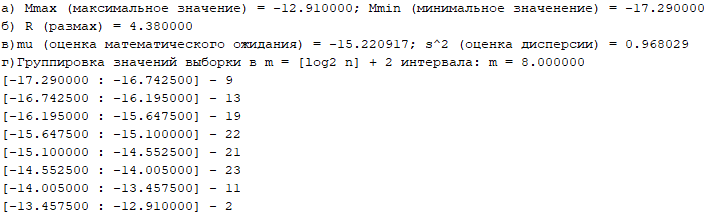
\includegraphics[scale=1]{inc/img/output.png}
\captionsetup{justification=centering}
	\caption{Поток вывода программы.}
	\label{img:output}	
\end{center}
\end{figure}

\item Гистограмма и график функции плотности распределения вероятностей нормальной случайной величины с математическим ожиданием $\hat \mu$ и дисперсией $S^2$ \ref{img:outputGraph}. 

\begin{figure}[H]
\begin{center}
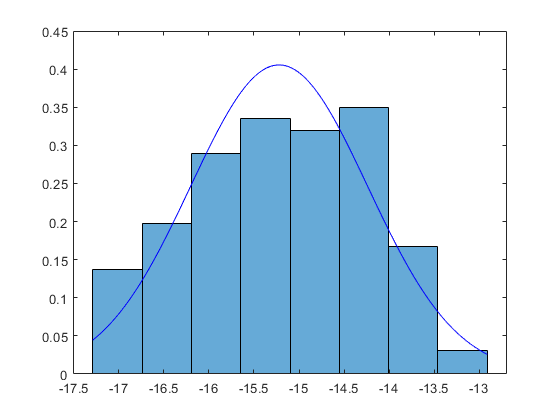
\includegraphics[scale=1]{inc/img/outputGraph.png}
\captionsetup{justification=centering}
	\caption{Гистограмма и график функции плотности распределения вероятностей нормальной случайной величины с математическим ожиданием $\hat \mu$ и дисперсией $S^2$.}
	\label{img:outputGraph}	
\end{center}
\end{figure}

\item График эмпирической функции распределения и функции распределения нормальной случайной величины с математическим ожиданием $\hat \mu$ и дисперсией $S^2$ \ref{img:outputGraph2}. 

\begin{figure}[H]
\begin{center}
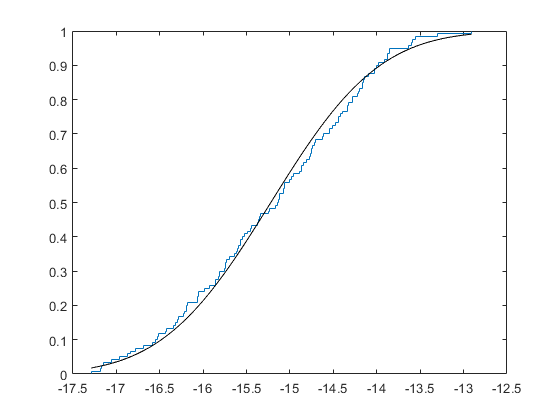
\includegraphics[scale=1]{inc/img/outputGraph2.png}
\captionsetup{justification=centering}
	\caption{График эмпирической функции распределения и функции распределения нормальной случайной величины с математическим ожиданием $\hat \mu$ и дисперсией $S^2$.}
	\label{img:outputGraph2}	
\end{center}
\end{figure}

\end{enumerate}
\end{document}